\newpage
\def\tenchude{GIÁ TRỊ LƯỢNG GIÁC CỦA MỘT GÓC}
\setcounter{dang}{0}
\chap{HỆ THỨC LƯỢNG TRONG TAM GIÁC}
\setcounter{section}{4}
\section{GTLG của một góc từ \boldmath $0^\circ$ đến $180^\circ$ \unboldmath}
\subsection{KIẾN THỨC TRỌNG TÂM}
\subsubsection{Giá trị lượng giác của một góc}
Với mỗi góc $\alpha\, \left(0^\circ \leq \alpha \leq 180^\circ\right)$ ta xác định được một điểm $M$ duy nhất trên nửa đường tròn đơn vị sao cho $\widehat{xOM}=\alpha$ và giả sử điểm $M$ có tọa độ $M(x_0;y_0)$.\\
\begin{center}
	\begin{tikzpicture}[scale=1.2, font=\footnotesize,line join=round, line cap=round, >=stealth,x=2cm,y=2cm]
		\def\x{0.5}
		\def\a{60}
		\pgfmathsetmacro{\y}{\x*tan(\a)}
		\draw[->] (-1.5,0)--(1.6,0) node [below]{$x$};
		\draw[->] (0,-0.3)--(0,1.3) node [left]{$y$};
		\node at (0,0) [below left]{$O$};
		\draw (1,0) arc (0:180:2cm);
		\fill (1,0) node[below]{$1$} circle(1pt);
		\fill (-1,0) node[below]{$-1$} circle(1pt);
		\fill (0,1) node[above left]{$1$} circle(1pt);
		%	\fill (\x,0) node[below]{$x_0$} circle(1pt);
		\fill (-\x,0) node[below]{$x_0$} circle(1pt);
		%	\fill (\a:1) node[above right]{$M$} circle(1pt);
		\fill (180-\a:1) node[above left]{$M$} circle(1pt);
		\fill (0,\y) node[right]{$y_0$} circle(1pt);
		\draw[dashed] (-\x,0)|-(0,\y);
		\draw (0,0)--(120:1);
		\draw (0.3,0) arc (0:180-\a:0.6cm);
		\node at (0,0)[shift={(25:0.2)}]{$\alpha$};
	\end{tikzpicture}
\end{center}
Khi đó ta có định nghĩa
\begin{khung4}{}
	\begin{multicols}{2}
		\begin{itemize}
			\item $\sin\alpha = y_0$.
			\item $\tan\alpha = \dfrac{y_0}{x_0}$ (với $x_0 \ne 0$).
			\item $\cos\alpha = x_0$.
			\item $\cot\alpha = \dfrac{x_0}{y_0}$ (với $y_0 \ne 0$).
		\end{itemize}
	\end{multicols}
\end{khung4}
Các số $\sin\alpha$, $\cos\alpha$, $\tan\alpha$, $\cot\alpha$ được gọi chung là các \textit{giá trị lượng giác} của góc $\alpha$.

\subsubsection{Mối quan hệ giữa các giá trị lượng giác của hai góc liên quan đặc biệt}
\begin{multicols}{2}
	\begin{khung4}{Hai góc phụ nhau}
		\begin{itemize}
			\item $\sin\left(90^{\circ}-\alpha\right)=\cos\alpha$.
			\item $\cos\left(90^{\circ}-\alpha\right)=\sin\alpha$.
			\item $\tan\left(90^{\circ}-\alpha\right)=\cot\alpha$.
			\item $\cot\left(90^{\circ}-\alpha\right)=\tan\alpha$.
		\end{itemize}
	\end{khung4}
	\begin{khung4}{Hai góc bù nhau}
		\begin{itemize}
			\item $\sin\left(180^{\circ}-\alpha\right)=\sin\alpha$.
			\item $\cos\left(180^{\circ}-\alpha\right)=-\cos\alpha$.
			\item $\tan\left(180^{\circ}-\alpha\right)=-\tan\alpha$.
			\item $\cot\left(180^{\circ}-\alpha\right)=-\cot\alpha$.
		\end{itemize}
	\end{khung4}

\end{multicols}
\subsubsection{Giá trị lượng giác của một số góc đặc biệt}
Dưới đây là bảng giá trị lượng giác của một số góc đặc biệt.
\begin{center}
	\renewcommand{\arraystretch}{2.1}%
	\begin{tabular}{|c|c|c|c|c|c|c|c|c|c|c|}
		\hline
		$\alpha$     & $0^\circ$   & $30^\circ$            & $45^\circ$            & $60^\circ$            & $90^\circ$  & $120^\circ$            & $135^\circ$            & $150^\circ$            & $180^\circ$ \\
		\hline
		$\sin\alpha$ & $0$         & $\dfrac{1}{2}$        & $\dfrac{\sqrt{2}}{2}$ & $\dfrac{\sqrt{3}}{2}$ & $1$         & $\dfrac{\sqrt{3}}{2}$  & $\dfrac{\sqrt{2}}{2}$  & $\dfrac{1}{2}$         & $0$         \\
		\hline
		$\cos\alpha$ & $1$         & $\dfrac{\sqrt{3}}{2}$ & $\dfrac{\sqrt{2}}{2}$ & $\dfrac{1}{2}$        & $0$         & $-\dfrac{1}{2}$        & $-\dfrac{\sqrt{2}}{2}$ & $-\dfrac{\sqrt{3}}{2}$ & $-1$        \\
		\hline
		$\tan\alpha$ & $0$         & $\dfrac{\sqrt{3}}{3}$ & $1$                   & $\sqrt{3}$            & $\parallel$ & $-\sqrt{3}$            & $-1$                   & $-\dfrac{\sqrt{3}}{3}$ & $0$         \\
		\hline
		$\cot\alpha$ & $\parallel$ & $\sqrt{3}$            & $1$                   & $\dfrac{\sqrt{3}}{3}$ & $0$         & $-\dfrac{\sqrt{3}}{3}$ & $-1$                   & $-\sqrt{3}$            & $\parallel$ \\
		\hline
	\end{tabular}
\end{center}
\subsection{PHÂN LOẠI VÀ PHƯƠNG PHÁP GIẢI TOÁN}

\begin{dang}{Tính các giá trị lượng giác của các góc cho trước}
	\begin{itemize}
		\item Dựa vào định nghĩa các giá trị lượng giác.
		\item Sử dụng các công thức lượng giác (công thức lượng giác cơ bản, công thức liên hệ các góc bù nhau, phụ nhau).
		\item Dấu của các giá trị lượng giác.
	\end{itemize}
	\begin{center}
		\renewcommand\arraystretch{1.2} %tăng độ rộng
		% \renewcommand{\tabcolsep}{6mm} %tăng chiều dài
		\begin{tabular}{|c|l l r|l r c|}
			\hline
			Góc $\alpha$ & $0^\circ$ &     & \multicolumn{2}{c}{$90^\circ$} &  & $180^\circ$   \\
			\hline
			$\sin\alpha$ &           & $+$ &                                &  & $+$         & \\
			\hline
			$\cos\alpha$ &           & $+$ &                                &  & $-$         & \\
			\hline
			$\tan\alpha$ &           & $+$ &                                &  & $-$         & \\
			\hline
			$\cot\alpha$ &           & $+$ &                                &  & $-$         & \\
			\hline
		\end{tabular}
	\end{center}
\end{dang}
\begin{vd}%[0H4N1-2]
	Sử dụng định nghĩa, tính các giá trị lượng giác của các góc $0^\circ $, $90^\circ $, $180^\circ $.
	\immini{\phantom{B}\dongcham{10}
	}{
		\begin{tikzpicture}[scale=1,line cap=round,line join=round,>=stealth,x=2cm,y=2cm]
			\draw[->] (-1.5,0)--(1.5,0) node[below] {$x$};
			\foreach \x in {-1,1}
			\draw[shift={(\x,0)},color=black] (0pt,1pt)--(0pt,-1pt)node[below]{$\x$};
			\draw[->,color=black] (0,-0.5)--(0,1.5) node[left] {$y$};
			\foreach \y in {1}
			\draw[shift={(0,\y)},color=black] (1pt,0pt)--(-1pt,0pt)node[above left] {$\y$};
			\fill (0,0) node[below left] {$O$} circle (1pt);
			\draw (-1,0) arc (180:0:1);
			\fill (-1,0) circle (1pt) node[above left] {$A'$};
			\fill (0,1) circle (1pt) node[above right] {$B$};
			\fill (1,0) circle (1pt) node[above right] {$A$};
		\end{tikzpicture}}
	\loigiai{
		\immini{\begin{itemize}
				\item Với $\alpha=0^\circ$. Khi đó, $M$ trùng với $A(1;0)$. Do đó, $\sin0^\circ=0$, $\cos0^\circ=1$, $\tan0^\circ=0$, $\cot0^\circ$ không xác định.
				\item Với $ \alpha=90^\circ$. Khi đó, $M$ trùng với $B(0;1)$. Do đó, $\sin90^\circ=1$, $\cos90^\circ=0$, $\tan90^\circ$ không xác định, $\cot90^\circ=0$.
			\end{itemize}
		}{
			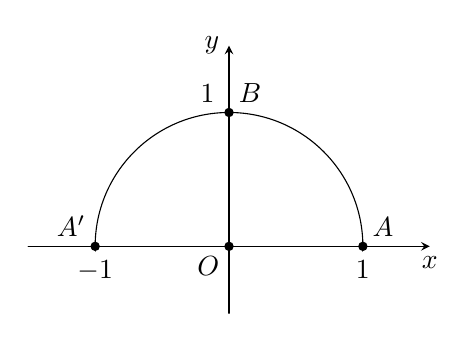
\begin{tikzpicture}[scale=1.7,line cap=round,line join=round,>=stealth]
				\draw[->] (-1.5,0)--(1.5,0) node[below] {$x$};
				\foreach \x in {-1,1}
				\draw[shift={(\x,0)},color=black] (0pt,1pt)--(0pt,-1pt)node[below]{$\x$};
				\draw[->,color=black] (0,-0.5)--(0,1.5) node[left] {$y$};
				\foreach \y in {1}
				\draw[shift={(0,\y)},color=black] (1pt,0pt)--(-1pt,0pt)node[above left] {\normalsize $\y$};
				\fill (0,0) node[below left] {\normalsize $O$} circle (1pt);
				\draw (-1,0) arc (180:0:1);
				\fill (-1,0) circle (1pt) node[above left] {$A'$};
				\fill (0,1) circle (1pt) node[above right] {$B$};
				\fill (1,0) circle (1pt) node[above right] {$A$};
			\end{tikzpicture}}
		\begin{itemize}
			\item Với $\alpha=180^\circ$. Khi đó, $M$ trùng với $A'(-1;0)$. Do đó, $\sin180^\circ=0$, $\cos180^\circ=-1$, $\tan180^\circ=0$, $\cot180^\circ$ không xác định.
		\end{itemize}
	}
\end{vd}

\begin{vd}%[0H4N1-2]
	Sử dụng định nghĩa, tìm các giá trị lượng giác của góc $135^\circ$.
	\immini{\dongcham{6}}
	{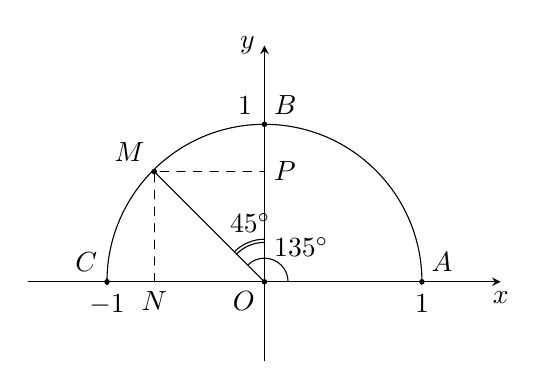
\begin{tikzpicture}[scale=1,x=2cm,y=2cm,line cap=round,line join=round,>=stealth]
			\draw[->] (-1.5,0) -- (1.5,0) node[below] {$x$};
			\foreach \x in {-1,1}
			\draw[shift={(\x,0)},color=black] (0pt,1pt)--(0pt,-1pt)node[below] { $\x$};
			\draw[->,color=black] (0,-0.5)--(0,1.5)  node[left] {$y$};
			\foreach \y in {1}
			\draw[shift={(0,\y)},color=black] (1pt,0pt)--(-1pt,0pt)node[above left] {\normalsize $\y$};
			\fill (0,0) node[below left] {\normalsize $O$} circle (1pt);
			\draw (-1,0) arc (180:0:1);
			\fill (-1,0) circle (1pt) node[above left] {$C$};
			\fill (0,1) circle (1pt) node[above right] {$B$};
			\fill (1,0) circle (1pt) node[above right] {$A$};
			\fill (-0.7,0.7) circle (1pt) node[above left] {$M$};
			\draw[dashed] (-0.7,0)--(-0.7,0.7)--(0,0.7);
			\node[below] at (-0.7,0) {$N$};
			\node[right] at (0,0.7) {$P$};
			\draw (0,0)--(-0.7,0.7);
			\draw (0.15,0) arc (0:135:0.15);
			\draw (0,0.25) arc (90:135:0.25);
			\draw (0,0.27) arc (90:135:0.27);
			\node[above right] at (0,0.1) {$135^\circ$};
			\node[above left] at (0.1,0.25) {$45^\circ$};
		\end{tikzpicture}}
	\loigiai{
		\immini{
			Gọi $M$ là điểm trên nửa đường tròn đơn vị sao cho $\widehat{xOM}=135^\circ$. Gọi $N$, $P$ tương ứng là hình chiếu vuông góc của $M$ lên các trục $Ox$, $Oy$.\\
			Vì $\widehat{xOM}=135^\circ$ nên $\widehat{MON}=45^\circ$, $\widehat{MOP}=45^\circ$. Vậy các tam giác $MON$, $MOP$ là vuông cân với cạnh huyền $ OM=1 $.
		}{
			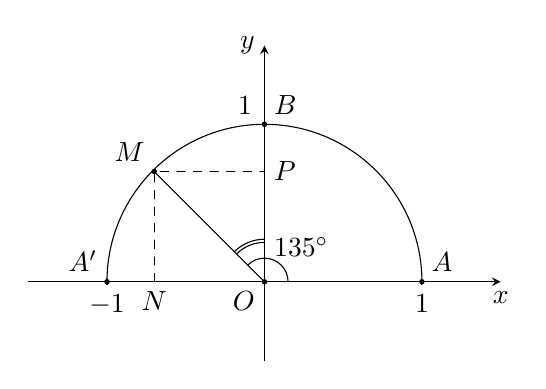
\begin{tikzpicture}[scale=1,x=2cm,y=2cm,line cap=round,line join=round,>=stealth]
				\draw[->] (-1.5,0) -- (1.5,0) node[below] {$x$};
				\foreach \x in {-1,1}
				\draw[shift={(\x,0)},color=black] (0pt,1pt)--(0pt,-1pt)node[below] { $\x$};
				\draw[->,color=black] (0,-0.5)--(0,1.5)  node[left] {$y$};
				\foreach \y in {1}
				\draw[shift={(0,\y)},color=black] (1pt,0pt)--(-1pt,0pt)node[above left] {\normalsize $\y$};
				\fill (0,0) node[below left] {\normalsize $O$} circle (1pt);
				\draw (-1,0) arc (180:0:1);
				\fill (-1,0) circle (1pt) node[above left] {$A'$};
				\fill (0,1) circle (1pt) node[above right] {$B$};
				\fill (1,0) circle (1pt) node[above right] {$A$};
				\fill (-0.7,0.7) circle (1pt) node[above left] {$M$};
				\draw[dashed] (-0.7,0)--(-0.7,0.7)--(0,0.7);
				\node[below] at (-0.7,0) {$N$};
				\node[right] at (0,0.7) {$P$};
				\draw (0,0)--(-0.7,0.7);
				\draw (0.15,0) arc (0:135:0.15);
				\draw (0,0.25) arc (90:135:0.25);
				\draw (0,0.27) arc (90:135:0.27);
				\node[above right] at (0,0.1) {$135^\circ$};
				% \node[above left] at (0.1,0.25) {$45^\circ$};
			\end{tikzpicture}}
		\noindent $ON=OP=\dfrac{\sqrt{2}}{2}$. Mặt khác, điểm $M$ nằm bên trái trục tung nên có tọa độ là $\left( -\dfrac{\sqrt{2}}{2};\dfrac{\sqrt{2}}{2}\right) $.\\
		Theo định nghĩa ta có
		\begin{listEX}[2]
			\item[$\bullet$] $\sin135^\circ=\dfrac{\sqrt{2}}{2}$;
			\item[$\bullet$] $\cos135^\circ=-\dfrac{\sqrt{2}}{2}$;
			\item[$\bullet$] $\tan135^\circ=-1$;
			\item[$\bullet$] $\cot135^\circ=-1$.
		\end{listEX}
	}
\end{vd}

\begin{vd}%[0H4N1-2]
	Dựa vào mối qan hệ hai góc bù nhau, tìm các giá trị lượng giác của góc $120^\circ$ dựa vào góc $60^\circ$.
	\dongcham{4}
	\loigiai{
		Ta có
		\begin{listEX}[2]
			\item[$\bullet$] $\sin120^\circ=\sin60^\circ=\dfrac{\sqrt{3}}{2}$;
			\item[$\bullet$] $\cos120^\circ=-\cos60^\circ=-\dfrac{1}{2}$;
			\item[$\bullet$] $\tan120^\circ=-\tan60^\circ=-\sqrt{3}$;
			\item[$\bullet$] $\cot120^\circ=-\cot60^\circ=-\dfrac{\sqrt{3}}{3}$.
		\end{listEX}
	}
\end{vd}
\begin{vd}%[0H2B1-2]%[Nguyễn Tiến]%Ví dụ 1.
	Tính các giá trị lượng giác của một góc, dựa vào một giá trị lượng giác cho trước.
	\begin{enumerate}
		\item Cho $\sin\alpha=\dfrac{1}{3}$ với $90^\circ<\alpha<180^\circ$. Tính $\cos\alpha$ và $\tan\alpha$, $\cot \alpha$. \dongcham{6}
		\item Cho $\cos\alpha=-\dfrac{2}{3}$. Tính $\sin\alpha$ và $\tan \alpha$, $\cot\alpha$.\dongcham{6}
		\item Cho $\tan\alpha=-2\sqrt{2}$, tính các giá trị lượng giác còn lại.\dongcham{6}
		\item Cho $\tan \alpha = \dfrac{1}{3}$, tính các giá trị lượng giác còn lại. \dongcham{6}
	\end{enumerate}
	\loigiai{
		\begin{enumerate}
			\item Vì $90^\circ<\alpha<180^\circ$ nên $\cos\alpha<0$, mặt khác $\sin^2\alpha+\cos^2\alpha=1$ suy ra
			      $$\cos\alpha=-\sqrt{1-\sin^2\alpha}=-\sqrt{1-\dfrac{1}{9}}=-\dfrac{2\sqrt{2}}{3}.$$
			      Do đó $\tan\alpha=\dfrac{\sin\alpha}{\cos\alpha}=\dfrac{\dfrac{1}{3}}{-\dfrac{2\sqrt{2}}{3}}=-\dfrac{1}{2\sqrt{2}}$.\\
			      $\cot \alpha = \dfrac{1}{\tan\alpha} = -2\sqrt{2}$.
			\item Vì $\sin^2\alpha+\cos^2\alpha=1$ và $\sin\alpha>0$, nên $\sin\alpha=\sqrt{1-\cos^2\alpha}=\sqrt{1-\dfrac{4}{9}}=\dfrac{\sqrt{5}}{3}$.\\
			      Ta có $\cot\alpha=\dfrac{\cos\alpha}{\sin\alpha}=\dfrac{-\dfrac{2}{3}}{\dfrac{\sqrt{5}}{3}}=-\dfrac{2}{\sqrt{5}}$.\\
			      $\tan\alpha = \dfrac{1}{\cot \alpha} =- \dfrac{\sqrt{5}}{2}$.
			\item Ta có $\cot \alpha = \dfrac{1}{\tan \alpha} = -\dfrac{1}{2\sqrt{2}}$\\
			      Vì $\tan\alpha=-2\sqrt{2}<0\Rightarrow\cos\alpha<0$.\\
			      Ta có $\tan^2\alpha+1=\dfrac{1}{\cos^2\alpha}$, suy ra $\cos\alpha=-\sqrt{\dfrac{1}{\tan^2+1}}=-\sqrt{\dfrac{1}{8+1}}=-\dfrac{1}{3}$.\\
			      Vì $\tan\alpha=\dfrac{\sin\alpha}{\cos\alpha}\Rightarrow\sin\alpha=\tan\alpha\cdot\cos\alpha=-2\sqrt{2}\cdot\left(-\dfrac{1}{3}\right)=\dfrac{2\sqrt{2}}{3}$.
			\item Ta có $\cot \alpha = \dfrac{1}{\tan \alpha} = 3$\\
			      Vì $\cot \alpha >0$ nên $\sin \alpha >0$.\\
			      Khi đó $\dfrac{1}{\sin ^2 \alpha}=1+\cot^2 \alpha = 1+3^2 =10$. Suy ra $\sin^2 \alpha = \dfrac{1}{10}$ nên $\sin \alpha = \sqrt{\dfrac{1}{10}}= \dfrac{\sqrt{10}}{10}$.\\
			      $\cot \alpha = \dfrac{\cos \alpha}{\sin \alpha} \Rightarrow \cos \alpha = \cot \alpha \cdot \sin \alpha = \dfrac{3\sqrt{10}}{10}$.
		\end{enumerate}
	}
\end{vd}
\begin{dang}{Tính giá trị các biểu thức lượng giác}
	Từ giả thiết đề cho (thường là giá trị của góc hay một giá trị lượng giác) định hướng biến đổi biểu thức về dạng chỉ xuất hiện giá trị đã cho của giả thiết để tính.
	\begin{note}
		Cần chú ý điều kiện áp dụng (nếu có).
	\end{note}
\end{dang}
\begin{vd}%[0H4H1-2]
	Tính $A=a\cos60^{\circ}+2a\tan45^{\circ}-3a\sin30^{\circ}$.
	\dongcham{1}
	\loigiai{
		Ta có $A=\dfrac{1}{2}a+2a-\dfrac{1}{2} \cdot 3a
			=a$.
	}
\end{vd}
%%=========
\begin{vd}%[0H4N1-2]
	Cho $x=30^{\circ}$. Tính $A=\sin 2x-3\cos x$.
	\dongcham{2}
	\loigiai{
		Ta có $A
			=\sin 2\cdot (30^{\circ})-3\cos30^{\circ}=\sin60^{\circ}-3\cos30^{\circ}=\dfrac{\sqrt{3}}{2}-3\dfrac{\sqrt{3}}{2}=-\sqrt{3}$.
	}
\end{vd}
\begin{vd}%[0H4N1-1]
	Cho góc $\alpha$ thỏa mãn $\cos \alpha=\dfrac{1}{3}$. Giá trị của biểu thức $P=\sin \alpha+\dfrac{1}{\cos \alpha}$ bằng\\
	\dongcham{4}
	\loigiai{
		Ta có $\sin ^2 \alpha+\cos ^2 \alpha=1 \Leftrightarrow \sin ^2 \alpha=1-\cos ^2 \alpha$.\\
		Với $\cos \alpha=\dfrac{1}{3} \Rightarrow \sin ^2 \alpha=1-\left(\dfrac{1}{3}\right)^2=\dfrac{8}{9} \Leftrightarrow \sin \alpha=\dfrac{2 \sqrt{2}}{3}$.\\
		Vậy $P=\sin \alpha+\dfrac{1}{\cos \alpha}=\dfrac{2 \sqrt{2}}{3}+\dfrac{1}{\tfrac{1}{3}}=\dfrac{2 \sqrt{2}}{3}+3=\dfrac{9+2 \sqrt{2}}{3}$.
	}
\end{vd}
\begin{vd}%[0H4N1-1]
	Cho biết $\sin \dfrac{\alpha}{3}=\dfrac{3}{5}$. Giá trị của $P=3 \sin ^2 \dfrac{\alpha}{3}+5 \cos ^2 \dfrac{\alpha}{3}$ bằng bao nhiêu?\\
	\dongcham{2}
	\loigiai{
		Ta có biểu thức $\sin ^2 \dfrac{\alpha}{3}+\cos ^2 \dfrac{\alpha}{3}=1 \Leftrightarrow \cos ^2 \dfrac{\alpha}{3}=1-\sin ^2 \dfrac{\alpha}{3}=\dfrac{16}{25}$.\\
		Do đó ta có $P=3 \sin ^2 \dfrac{\alpha}{3}+5 \cos ^2 \dfrac{\alpha}{3}=3 \cdot\left(\dfrac{3}{5}\right)^2+5 \cdot \dfrac{16}{25}=\dfrac{107}{25}$.
	}
\end{vd}
\begin{vd}%[0H4N1-1]
	Cho $\tan \alpha=2$. Giá trị của $A=\dfrac{3 \sin \alpha+\cos \alpha}{\sin \alpha-\cos \alpha}$ là
	\dongcham{4}
	\loigiai{
		Ta có $A=\dfrac{3 \sin \alpha+\cos \alpha}{\sin \alpha-\cos \alpha}=\dfrac{3 \tan \alpha+1}{\tan \alpha-1}=\dfrac{3\cdot 2+1}{2-1}=7$.
	}
\end{vd}

\begin{dang}{Chứng minh đẳng thức lượng giác}
	Sử dụng linh hoạt các công thức cở bản, các phép biến đổi đại
	số và sử dụng các hằng đẳng thức đáng nhớ để rút gọn và chứng minh.
\end{dang}
\begin{vd}%[0H4H1-2]
	Cho $\heva{&a=\sin x\\&b=\cos x\sin x\\&c=\cos x\cos y}$. Chứng minh rằng $a^2+b^2+c^2=1$
	\dongcham{3}
	\loigiai{Ta có:
		\begin{align*}
			a^2+b^2+c^2 & =\sin^2x+\cos^2x(1-\cos^2y)+\cos^2x\cos^2y     \\
			            & =\sin^2x+\cos^2x-\cos^2x\cos^2y+\cos^2x\cos^2y \\
			            & =1.
		\end{align*}
	}
\end{vd}
%%==========
\begin{vd}%[0H4H1-2]
	Chứng minh các đẳng thức sau:
	\begin{enumerate}
		\item $\sin^4x+\cos^4x=1-2\sin^2x\cos^2x.$ \dongcham{4}
		\item $\cos^4x-\sin^4x=\cos^2x-\sin^2x=1-2\sin^2x=2\cos^2x-1.$\dongcham{8}
		\item $\tan^2x-\sin^2x=\tan^2x\sin^2x.$\dongcham{4}
		\item $\dfrac{1}{1+\tan x}+\dfrac{1}{1+\cot x}=1.$\dongcham{4}
	\end{enumerate}
	\loigiai{
		\begin{enumerate}
			\item Ta có $\sin^4x+\cos^4x=\left(\sin^2x\right)^2+\left(\cos^2x\right)^2= \left(\sin^2x+\cos^2x\right)^2-2\sin^2x\cos^2x$\\
			      Do $\sin^2x+\cos^2x=1$ nên ta suy ra $\sin^4x+\cos^4x=1-2\sin^2x\cos^2x.$
			\item $\cos^4x-\sin^4x=\left(\cos^2x\right)^2-\left(\sin^2x\right)^2=\left(\cos^2x-\sin^2x\right)\left(\cos^2x+\sin^2x\right)=\cos^2x-\sin^2x$\\
			      Do $\sin^2x+\cos^2x=1$ nên $\cos^2x-\sin^2x=\cos^2x+\sin^2x-2\sin^2x=1-2\sin^2x$\\
			      Tương tự ta có $\cos^2x-\sin^2x=2\cos^2x-1.$
			\item $\tan^2x-\sin^2x=\dfrac{\sin^2x}{\cos^2x}-\sin^2x=\sin^2x\left(\dfrac{1}{\cos^2x}-1\right)=\sin^2x\dfrac{1-\cos^2x}{\cos^2x}=\tan^2x\sin^2x$
			\item Ta có $\dfrac{1}{1+\tan x}+\dfrac{1}{1+\cot x}=\dfrac{1+\tan x+1+\cot x}{\left(1+\tan x\right)\left(1+\cot x\right)}$.\\
			      Mặt khác $\left(1+\tan x\right)\left(1+\cot x\right)=1+\tan x\cot x+\tan x+\cot x=2+\tan x+\cot x$.\\
			      Từ đó suy ra $\dfrac{1}{1+\tan x}+\dfrac{1}{1+\cot x}=\dfrac{2+\tan x+\cot x}{2+\tan x+\cot x}=1.$
		\end{enumerate}
	}
\end{vd}
\subsection{BÀI TẬP RÈN LUYỆN}
\baitaptl
\setcounter{bt}{0}
\begin{bt}%[0H4N1-2]
	Chứng minh rằng
	\begin{multicols}{2}
		\begin{enumerate}
			\item $\sin 20^\circ=\sin 160^\circ$;
			\item $\cos50^\circ=-\cos130^\circ$.
		\end{enumerate}
	\end{multicols}
	\loigiai{
		\begin{enumerate}
			\item Ta có $20^\circ+160^\circ=180^\circ$ nên $\sin 20^\circ=\sin 160^\circ$.
			\item Ta có $50^\circ+130^\circ=180^\circ$ nên $\cos50^\circ=-\cos130^\circ$.
		\end{enumerate}
	}
\end{bt}
\begin{bt}%[0H4H1-2]
	Cho góc $\alpha$ với $\cos\alpha=-\dfrac{\sqrt{2}}{2}$. Tính giá trị của biểu thức $A=2\sin^2\alpha+5\cos^2\alpha$.
	\loigiai{ Do $\cos\alpha=-\dfrac{\sqrt{2}}{2}$ mà $\cos^2\alpha+\sin^2\alpha=1$ nên $\sin^2\alpha=1-\left(-\dfrac{\sqrt{2}}{2} \right)^2=\dfrac{1}{2} $.\\
		Vậy $A=2\cdot \dfrac{1}{2}+5\cdot \dfrac{1}{2}=\dfrac{7}{2} $.
	}
\end{bt}
\begin{bt}%[0H4H1-3]
	Cho biết $\sin 30^\circ=\dfrac{1}{2}$; $\sin 60^\circ=\dfrac{\sqrt{3}}{2}$; $\tan 45^\circ=1$. Sử dụng mối liên hệ giữa các giá trị lượng giác của hai góc bù nhau, phụ nhau để tính giá trị của $E=2\cos30^\circ+\sin 150^\circ+\tan135^\circ$.
	\loigiai{
		Ta có $\cos30^\circ=\sin 60^\circ=\dfrac{\sqrt{3}}{2}$; $\sin150^\circ=\sin 30^\circ=\dfrac{1}{2}$; $\tan 135^\circ=-\tan45^\circ=-1$.\\
		Vậy
		\[E=2\cos30^\circ+\sin 150^\circ+\tan135^\circ=2\cdot\dfrac{\sqrt{3}}{2}+\dfrac{1}{2}+(-1)=\sqrt{3}-\dfrac{1}{2}.\]
	}
\end{bt}
%Bài 10
\begin{bt}%[0H4V1-2]
	\immini{Cột cờ Lũng Cú là cột cờ Quốc gia, nằm ở đỉnh Lũng Cú hay còn gọi là đỉnh Núi Rồng (Long Sơn) thuộc xã Lũng Cú, huyện Đồng Văn, tỉnh Hà Giang, cách cực Bắc Việt Nam khoảng $3{,}3$ km. Thời nhà Lý, cột cờ Lũng Cú chỉ được làm bằng cây sa mộc. Ngày nay, cột cờ có độ cao $33{,}15$ m bao gồm bệ cột cao $20{,}25$ m và cán cờ cao $12{,}9$ m. Chân bệ cột cờ có $8$ mặt phù điêu bằng đá xanh mô phỏng hoa văn mặt của trống đồng Đông Sơn và những họa tiết minh họa các giai đoạn qua từng thời kì lịch sử của đất nước, cũng như con người, tập quán của các dân tộc ở Hà Giang. Trên đỉnh cột là Quốc kì Việt Nam có diện tích $54$ m$^2$, biểu tượng cho $54$ dân tộc của đất nước ta.
		\begin{flushright}
			\textit{(Nguồn: http://baophutho.vn)}
		\end{flushright}
	}{
		\begin{tikzpicture}[font=\footnotesize, scale=1, line join =round, line cap= round, >= stealth, declare function={goc=50;a=4;k=a-.5;}]
			\path
			(0,0) coordinate (C)
			(a,0) coordinate (H)
			($(H)+(90:a)$) coordinate (A)
			(goc:1) coordinate (C1)
			(intersection of C--C1 and H--A) coordinate (B)
			($(A)+(180:k)$) coordinate (Ax)node[above]{$y$}
			($(B)+(180:k)$) coordinate (Bx) node[above]{$x$}
			;
			\draw (A)--(B)--(C)--cycle (A)--(H)--(C) (A)--(Ax) (B)--(Bx);
			\draw[<->,dashed] ($(H)+(0:.5)$)--($(A)+(0:.5)$) node[midway, right] {$h$};
			\path (A)--(B) node[right,pos=0.5]{$20{,}25$ m};
			\foreach \x/\g in {A/0,B/60,C/-90,H/-90} {
					\fill (\x) node[shift={(\g:7pt)}]{$\x$} circle (1pt);}
			\draw pic[draw,double,angle radius=4mm,angle eccentricity=1.7,"$50^\circ$"] {angle = Bx--B--C};
			\draw pic[draw,angle radius=3mm,angle eccentricity=2,"$45^\circ$"] {angle = Ax--A--C};
		\end{tikzpicture}
	}
	Từ chân bệ cột cờ và đỉnh bệ cột cờ bạn Nam đo được góc nâng (so với phương nằm ngang) tới một vị trí dưới chân núi lần lượt là $45^\circ$ và $50^\circ$ (xem hình minh hoạ bên). Tính chiều cao $h$ của đỉnh Lủng Cú so với chân núi (\textit{kết quả làm tròn hàng đơn vị của mét})?
	\loigiai{
		Ta có $Bx \parallel  CH \Rightarrow \widehat{BCH} = \widehat{xBC} = 50^\circ$ (hai góc so le trong).\\
		$Ay \parallel  CH \Rightarrow \widehat{ACH} = \widehat{yAC} = 45^\circ$ (hai góc so le trong).\\
		Tam giác $ACH$ vuông tại $H$ có $\widehat{ACH} = 45^\circ$ nên tam giác $ACH$ vuông cân tại $H$.\\
		Suy ra $CH = AH = h$ (m).\\
		Ta có $BH = AB + AH = 20{,}25 + h$.\\
		Tam giác $BCH$ vuông tại $H$ nên $\tan\widehat{BCH} = \dfrac{BH}{CH}$.\\
		Do đó ta có \[\tan 50^\circ=\dfrac{20{,}25+h}{h}\Leftrightarrow h=\dfrac{20{,}25}{\tan 50^\circ-1}\approx 106\,\text{(m).}\]
		Vậy chiều cao $h$ của đỉnh Lũng Cú so với chân núi là $106$ m.
	}
\end{bt}
\baitaptn
\ind{PHẦN I.} \inden{Câu trắc nghiệm nhiều phương án lựa chọn. Mỗi câu hỏi học sinh chỉ chọn một phương án.}
\setcounter{ex}{0}
\Opensolutionfile{ans}[ans/ansc3b5nlc]
\begin{ex}%[0H4N1-1]
	\immini{Trên nửa đường tròn đơn vị cho điểm $M$ sao cho $\widehat{xOM}=\alpha$ như hình vẽ bên. Khẳng định nào sau đây đúng?
		\choice[2]
		{\True $\sin \alpha>0$}
		{$\sin \alpha<0$}
		{$\sin \alpha=0$}
		{$\sin \alpha=1$}
	}{
		\begin{tikzpicture}[scale=1, font=\footnotesize,
				line join=round, line cap=round, >=stealth,
				declare function={
						r=2;
						goc=60;
						xm=r*cos(goc);
						ym=r*sin(goc);
					}]
			\path (r,0) coordinate (A) (xm,ym) coordinate (M) (0,0) coordinate (O);
			\draw[->] (-.5-r,0)--(r+0.5,0) node [below]{$x$};
			\draw[->] (0,-0.5)--(0,r+0.5) node [left]{$y$};
			\fill (O) circle (1pt) node[shift={(-135:7pt)}]{$O$};
			\draw (r,0) arc (0:180:r);
			\fill (r,0) node[below]{$1$} circle(1pt);
			\fill (-r,0) node[below]{$-1$} circle(1pt);
			\fill (0,r) node[above right]{$1$} circle(1pt);
			\fill (xm,ym) node[shift={(goc:7pt)}]{$M$} circle(1pt);
			\draw (O)--(M)
			pic[draw,angle radius=3mm,angle eccentricity=2,"$\alpha$"] {angle = A--O--M};
		\end{tikzpicture}
	}
	\loigiai{
		Giá trị $\sin \alpha$ là tung độ của điểm $M$ nên suy ra $\sin \alpha>0$.
	}
\end{ex}
%câu 2
\begin{ex}%[0H4N1-1]
	\immini{Trên nửa đường tròn đơn vị cho điểm $M$ sao cho $\widehat{xOM}=\alpha$ như hình vẽ bên. Khẳng định nào sau đây đúng?
		\choice[2]
		{$\cos \alpha>0$}
		{\True $\cos \alpha<0$}
		{$\cos \alpha=0$}
		{$\cos \alpha=1$}
	}{
		\begin{tikzpicture}[scale=1, font=\footnotesize,
				line join=round, line cap=round, >=stealth,
				declare function={
						r=2;
						goc=130;
						xm=r*cos(goc);
						ym=r*sin(goc);
					}]
			\path (r,0) coordinate (A) (xm,ym) coordinate (M) (0,0) coordinate (O);
			\draw[->] (-.5-r,0)--(r+0.5,0) node [below]{$x$};
			\draw[->] (0,-0.5)--(0,r+0.5) node [left]{$y$};
			\fill (O) circle (1pt) node[shift={(-135:7pt)}]{$O$};
			\draw (r,0) arc (0:180:r);
			\fill (r,0) node[below]{$1$} circle(1pt);
			\fill (-r,0) node[below]{$-1$} circle(1pt);
			\fill (0,r) node[above right]{$1$} circle(1pt);
			\fill (xm,ym) node[shift={(goc:7pt)}]{$M$} circle(1pt);
			\draw (O)--(M)
			pic[draw,angle radius=3mm,angle eccentricity=2,"$\alpha$"] {angle = A--O--M};
		\end{tikzpicture}
	}
	\loigiai{
		Giá trị $\cos \alpha$ là hoành độ của điểm $M$ nên suy ra $\cos \alpha<0$.
	}
\end{ex}
%câu 3
\begin{ex}%[0H4N1-2]
	Cho góc $\widehat{xOM}=\alpha$ với điểm $M\left(\dfrac{1}{3}; \dfrac{2\sqrt{2}}{3}\right)$ trên nửa đường tròn đơn vị. Giá trị lượng giác của $\tan \alpha$ là
	\choice
	{$\tan \alpha=-\dfrac{2\sqrt{2}}
			{1}$}
	{\True $\tan \alpha=-2\sqrt{2}$}
	{$\tan \alpha=\dfrac{2\sqrt{2}-1}{3}$}
	{$\tan \alpha=\dfrac{2\sqrt{2}}{9}$}
	\loigiai{
		Ta thấy $M\left(\dfrac{1}{3}; \dfrac{2\sqrt{2}}{3}\right)$, suy ra
		$\cos \alpha=\dfrac{1}{3}$,
		$\sin \alpha=\dfrac{2\sqrt{2}}{3}$.\\
		$\Rightarrow \tan \alpha=\dfrac{\sin \alpha}{\cos \alpha}=\dfrac{\dfrac{2\sqrt{2}}{3}}{\dfrac{1}{3}}=2\sqrt{2}$.
	}
\end{ex}
%câu 4
\begin{ex}%[0H4N1-2]
	Cho góc $\widehat{xOM}=\alpha$ với điểm $M\left(\dfrac{1}{3}; \dfrac{2\sqrt{2}}{3}\right)$ trên nửa đường tròn đơn vị. Giá trị lượng giác của $\cot \alpha$ là
	\choice
	{\True $\cot \alpha=\dfrac{1}
			{2\sqrt{2}}$}
	{$\cot \alpha=2\sqrt{2}$}
	{$\cot \alpha=\dfrac{2\sqrt{2}-1}{3}$}
	{$\cot \alpha=\dfrac{2\sqrt{2}}{9}$}
	\loigiai{
		Ta thấy $M\left(\dfrac{1}{3}; \dfrac{2\sqrt{2}}{3}\right)$ suy ra
		$\cos \alpha=\dfrac{1}{3}$,
		$\sin \alpha=\dfrac{2\sqrt{2}}{3}$.\\
		$\Rightarrow \cot \alpha=\dfrac{\cos \alpha}{\sin \alpha}=\dfrac{\dfrac{1}{3}}{\dfrac{2\sqrt{2}}{3}}=\dfrac{1}{2\sqrt{2}}$.
	}
\end{ex}
\begin{ex}%[0H4N1-1]
	Cho $0^{\circ}  < \alpha < 90^{\circ} $. Khẳng định nào sau đây đúng?
	\choice
	{$\cot \left(90^{\circ} -\alpha \right)=-\tan \alpha$}
	{\True $\cos \left(90^{\circ} -\alpha \right)=\sin \alpha$}
	{$\sin \left(90^{\circ} -\alpha \right)=-\cos \alpha$}
	{$\tan \left(90^{\circ} -\alpha \right)=-\cot \alpha$}
	\loigiai{
		Vì $\alpha$ và $\left(90^{\circ} -\alpha \right)$ là hai cung phụ nhau nên $\cos \left(90^{\circ} -\alpha \right)=\sin \alpha$.
	}
\end{ex}%[0H4N1-2]
%%%==============
\begin{ex}%[0H4H1-2]
	Tính giá trị biểu thức $P=\sin 30^{\circ} \cos 60^{\circ}+\sin 60^{\circ} \cos 30^{\circ}$
	\choice
	{\True $P=1$}
	{$P=0$}
	{$P=\sqrt{3}$}
	{$P=-\sqrt{3}$}
	\loigiai{
		Ta có $P=\sin 30^{\circ} \cdot \sin 30^{\circ}+\cos 30^{\circ} \cdot \cos 30^{\circ}=\sin^2 30^{\circ}+\cos^2 30^{\circ}=1$.
	}
\end{ex}
%%%==============
\begin{ex}%[0H4H1-1]
	Biết $A$, $B$, $C$ là ba góc của tam giác $ABC$, mệnh đề nào sau đây là đúng?
	\choice
	{$\cos \left(A+C\right)=\cos B$}
	{\True $\tan \left(A+C\right)=-\tan B$}
	{$\cot \left(A+C\right)=\cot B$}
	{$\sin \left(A+C\right)=-\sin B$}
	\loigiai{
		\begin{itemize}
			\item Xét đáp án $\cos \left(A+C\right)=\cos \left(180^\circ-B\right)=-\cos B \Rightarrow$ đáp án sai.
			\item Xét đáp án $\tan \left(A+C\right)=\tan \left(\pi-B\right)=-\tan B$ nên là đáp án đúng.
			\item Xét đáp án $\cot \left(A+C\right)=\cot \left(\pi-B\right)=-\cot B \Rightarrow$ đáp án sai.
			\item Xét đáp án $\sin \left(A+C\right)=\sin \left(\pi-B\right)=\sin B \Rightarrow$ đáp án sai.
		\end{itemize}
	}
\end{ex}
\begin{ex}%[0H4N1-1]
	Cho $\alpha$ là góc tù. Điều khẳng định nào sau đây là đúng?
	\choice
	{$\sin \alpha < 0$}
	{$\cos \alpha > 0$}
	{\True $\tan \alpha < 0$}
	{$\cot \alpha > 0$}
	\loigiai{
		Góc tù có điểm biểu diễn thuộc góc phần tư thứ II, có giá trị $\sin \alpha > 0$, còn $\cos \alpha$, $\tan \alpha$ và $\cot \alpha$ đều nhỏ hơn $0$.
	}
\end{ex}
\begin{ex}%[0H4N1-1]
	Trong các đẳng thức sau, đẳng thức nào đúng?
	\choice
	{$\sin \left(180^{\circ}-\alpha \right)=\cos \alpha$}
	{$\sin \left(180^{\circ}-\alpha \right)=-\cos \alpha$}
	{$\sin \left(180^{\circ}-\alpha \right)=-\sin \alpha$}
	{\True $\sin \left(180^{\circ}-\alpha \right)=\sin \alpha$}
	\loigiai{
		Vì hai góc $\alpha$ và $180^\circ - \alpha$ là hai góc bù nhau.
	}
\end{ex}
\begin{ex}%[0H4V1-2]
	Tam giác đều $ABC$ có đường cao $AH$. Khẳng định nào sau đây là đúng?
	\choice
	{$\cos \widehat{BAH}=\dfrac{1}
			{\sqrt{3}}$}
	{\True $\sin \widehat{ABC}=\dfrac{\sqrt{3}}
			{2}$}
	{$\sin \widehat{AHC}=\dfrac{1}{2}$}
	{$\sin \widehat{BAH}=\dfrac{\sqrt{3}}{2}$}
	\loigiai{
		Tam giác $ABC$ là tam giác đều nên có các góc bằng $60^{\circ}$ nên ta có
		\[\sin \widehat{ABC}=\sin 60^{\circ}=\dfrac{\sqrt{3}}{2}.
		\]
	}
\end{ex}
\begin{ex}%[0H4H1-2]
	Tam giác $ABC$ vuông ở $A$ có góc $\widehat{B}=30^{\circ}$. Khẳng định nào sau đây là sai?
	\choice
	{\True $\cos B=\dfrac{1}
			{\sqrt{3}}$}
	{$\sin C=\dfrac{\sqrt{3}}
			{2}$}
	{$\cos C=\dfrac{1}{2}$}
	{$\sin B=\dfrac{1}{2}$}
	\loigiai{
		Dễ thấy đáp án $\cos B=\dfrac{1}{\sqrt{3}}$ sai do $\cos B=\cos 30^{\circ}=\dfrac{\sqrt{3}}{2}$.
	}
\end{ex}
\begin{ex}%[0H4N1-2]
	Trong các đẳng thức sau đây đẳng thức nào là đúng?
	\choice
	{$\sin 150^{\circ}=-\dfrac{\sqrt{3}}
			{2}$}
	{$\cos 150^{\circ}=\dfrac{\sqrt{3}}
			{2}$}
	{\True $\tan 150^{\circ}=-\dfrac{1}{\sqrt{3}}$}
	{$\cot 150^{\circ}=\sqrt{3}$}
	\loigiai{
		Dựa vào giá trị lượng giác của các cung bù nhau. Dễ thấy phương án đúng là
		$\sin 150^{\circ}=\sin 30^{\circ}=\dfrac{1}{2}$,
		$\cos 150^{\circ}=-\cos 30^{\circ}=-\dfrac{\sqrt{3}}{2}$,
		$\tan 150^{\circ}=-\tan 30^{\circ}=-\dfrac{1}{\sqrt{3}}$ và $\cot 150^{\circ}=-\cot 30^{\circ}=-\sqrt{3}$.
	}
\end{ex}
\begin{ex}%[0H4H1-2]
	Cho góc $\alpha \in \left(90^{\circ};180^{\circ} \right)$. Khẳng định nào sau đây đúng?
	\choice
	{$\sin \alpha$ và $\cot \alpha$ cùng dấu}
	{\True Tích $\sin \alpha \cdot \cot \alpha$ mang dấu âm}
	{Tích $\sin \alpha  \cdot \cos \alpha$ mang dấu dương}
	{$\sin \alpha$ và $\tan \alpha$ cùng dấu}
	\loigiai{
		Với $\alpha \in \left(90^{\circ};180^{\circ} \right)$, ta có $\sin \alpha > 0,\cos \alpha < 0$ suy ra: $\tan \alpha < 0,\cot \alpha < 0$
		Vậy $\sin \alpha \cdot \cot \alpha < 0$
	}
\end{ex}
\begin{ex}%[0H4N1-2]
	Hai góc nhọn $\alpha$ và $\beta$ phụ nhau, hệ thức nào sau đây là sai?
	\choice
	{$\sin \alpha=\cos \beta$}
	{$\tan \alpha=\cot \beta$}
	{$\cot \beta=\dfrac{1}
			{\cot \alpha}$}
	{\True $\cos \alpha=-\sin \beta$}
	\loigiai{
		Ta có
		\[\cos \alpha=\cos \left(90^{^{\circ}}-\beta \right)=\sin \beta.
		\]
	}
\end{ex}
\begin{ex}%[0H4V1-2]
	Cho $\sin \alpha=\dfrac{1}{3}$, với $90^{\circ} < \alpha < 180^{\circ}$. Tính $\cos \alpha$.
	\choice
	{$\cos \alpha=\dfrac{2}
			{3}$}
	{$\cos \alpha=-\dfrac{2}
			{3}$}
	{$\cos \alpha=\dfrac{2\sqrt{2}}{3}$}
	{\True $\cos \alpha=-\dfrac{2\sqrt{2}}{3}$}
	\loigiai{
		Ta có $\cos^2 \alpha=1-\sin^2 \alpha$ $=1-\left(\dfrac{1}{3} \right)^2=\dfrac{8}{9}$.
		Mặt khác $90^{\circ} < \alpha < 180^{\circ}$ nên $\cos \alpha=-\dfrac{2\sqrt{2}}{3}$.
	}
\end{ex}
\begin{ex}%[0D3N1-2] %5
	Trong các đẳng thức sau, đẳng thức nào đúng?
	\choice
	{ $\sin \left(180^\circ-\alpha\right) = \cos \alpha $}
	{ $\sin \left( 180^\circ -\alpha \right) =  - \cos \alpha $}
	{$\sin \left( 180^\circ-\alpha \right) =  - \sin \alpha $}
	{\True $\sin \left( 180^\circ - \alpha  \right) = \sin \alpha $}
	\loigiai{ Vì $\alpha$ và $180^\circ - \alpha$ là hai cung bù nhau nên theo tính chất giá trị lượng giác của hai cung bù nhau ta có đáp án.
	}
\end{ex}
\begin{ex}%[0D3N1-2] %6
	Cho  $\alpha$ là góc tù. Điều khẳng định nào sau đây là đúng?.
	\choice
	{ $\sin \alpha  < 0$}
	{ $\cos \alpha  > 0$}
	{\True $\tan \alpha  < 0$}
	{$\cot \alpha  > 0$}
	\loigiai{ Dựa vào giá trị lượng giá của cung tư $0^\circ$ đến $180^\circ$. Suy ra $\sin \alpha >0; \cos \alpha <0$ với $\alpha$ là góc tù, nên $\tan \alpha= \dfrac{\sin \alpha}{\cos \alpha} <0$.
	}
\end{ex}
\begin{ex}%[0D3N1-2] %1
	Cho $0^\circ < \alpha < 90^\circ$. Khẳng định nào sau đây là đúng?
	\choice
	{ $\cot(90^\circ-\alpha)=-\tan\alpha$}
	{\True $\cos(90^\circ -\alpha = \sin \alpha)$}
	{$\sin(90^\circ - \alpha) =-\cos\alpha$}
	{$\tan(90^\circ-\alpha)= - \cot \alpha$}
	\loigiai{
		Vì $\alpha$ và $90^\circ - \alpha$ là hai cung phụ nhau nên theo tính chất giá trị lượng giác của hai cung phụ nhau ta có đáp án. }
\end{ex}
\begin{ex}%[0D3N1-2] %2
	Tính giá trị biểu thức  $P = \sin 30^\circ \cos 60^\circ  + \sin 60^\circ \cos 30^\circ $.
	\choice
	{ \True $P=1$}
	{ $P=0$}
	{$P=\sqrt{3}$}
	{$P=-\sqrt{3}$}
	\loigiai{
		Ta có $P = \sin 30^\circ .\sin 30^\circ  + \cos 30^\circ .\cos30^\circ  = {\sin ^2}30^\circ  + {\cos ^2}30^\circ  = 1$. }
\end{ex}
\Closesolutionfile{ans}
\indapan{6}{ans/ansc3b5nlc}
\ind{PHẦN II.} \inden{Câu trắc nghiệm đúng sai. Trong mỗi ý a), b), c), d) ở mỗi câu, học sinh chọn đúng hoặc sai.}
\setcounter{ex}{0}
\Opensolutionfile{ans}[ans/ansc3b5ds]
\begin{ex}%[0H4H1-2]
	Cho góc $\alpha=\widehat{xOM}$ với điểm $M(x_0; y_0)$ trên nửa đường tròn đơn vị.
	\choiceTF
	{Nếu $90<\alpha<180^\circ$ thì $\cos \alpha >0$}
	{Nếu $x_0 < 0$ thì $0^\circ < \alpha < 90^\circ$}
	{\True Nếu $x_0=\dfrac{1}{3}$; $ y_0=\dfrac{2\sqrt{2}}{3}$ thì giá trị $\cot \alpha=\dfrac{1}{2\sqrt{2}}$}
	{\True Nếu $x_0=-\dfrac{1}{3}$; $ y_0=\dfrac{2\sqrt{2}}{3}$ thì giá trị $\dfrac{\tan \alpha-\cot \alpha}{\tan \alpha+\cot \alpha}=\dfrac{7}{9}$}
	\loigiai{
		\begin{itemchoice}
			\itemch Nếu $90<\alpha<180^\circ$ thì $\cos \alpha <0$.
			\itemch Với $x_0 < 0$ thì $90^\circ < \alpha < 180^\circ$.
			\itemch Ta có
			$\sin \alpha=y_0=\dfrac{2\sqrt{2}}{3}$, $\cos \alpha=x_0=\dfrac{1}{3} \Rightarrow \cot \alpha=\dfrac{\cos \alpha}{\sin \alpha}=\dfrac{\dfrac{1}{3}}{\dfrac{2\sqrt{2}}{3}}=\dfrac{1}{2\sqrt{2}}$.
			\itemch Ta có $\sin \alpha=y_0=\dfrac{2\sqrt{2}}{3}$, $\cos \alpha=x_0=-\dfrac{1}{3}$.\\
			$\Rightarrow \cot \alpha=\dfrac{\cos \alpha}{\sin \alpha}=\dfrac{-\dfrac{1}{3}}{\dfrac{2\sqrt{2}}{3}}=-\dfrac{1}{2\sqrt{2}}$, $\tan \alpha=-2\sqrt{2}$.\\
			Vậy $\dfrac{\tan \alpha-\cot \alpha}{\tan \alpha+\cot \alpha}=\dfrac{-2\sqrt{2}+\dfrac{1}{2\sqrt{2}}}{-2\sqrt{2}-\dfrac{1}{2\sqrt{2}}}=\dfrac{7}{9}$.
		\end{itemchoice}
	}
\end{ex}
\begin{ex}%[0H4H1-2]
	Cho $\cos \alpha=\dfrac{1}{3}$ và $0^\circ < \alpha < 90^\circ$.
	\choiceTF
	{\True $\tan \alpha > 0$}
	{$\sin\left(90^\circ+\alpha\right)=\dfrac{2}{3}$}
	{\True $\tan \alpha=2\sqrt{2}$}
	{\True $\dfrac{1+\sin^2 \alpha}{1-\sin^2 \alpha}=1+2\tan^2 \alpha$}
	\loigiai{
		\begin{itemchoice}
			\itemch Vì $0^\circ < \alpha < 90^\circ$ nên $\tan \alpha > 0$.
			\itemch Ta có $\sin \left(90^\circ+\alpha\right)
				=\sin\left(180^\circ-\left(90^\circ+\alpha\right)\right)
				=\sin\left(90^\circ-\alpha\right)=\cos \alpha=\dfrac{1}{3}$.
			\itemch Ta có $1+\tan^2 \alpha=\dfrac{1}{\cos^2 \alpha}= \dfrac{1}{\left(\dfrac{1}{3}\right)^2}=9\Leftrightarrow \tan^2 \alpha=8 \Leftrightarrow \tan \alpha=2\sqrt{2}$ (vì $\tan \alpha>0$).
			\itemch Ta có $\dfrac{1+\sin^2 \alpha}{1-\sin^2 \alpha}=\dfrac{1+\sin^2 \alpha}{\cos^2 \alpha}=\dfrac{1}{\cos^2 \alpha}+\dfrac{\sin^2 \alpha}{\cos^2 \alpha}=\left(1+\tan^2 \alpha\right)+\tan^2 \alpha=1+2\tan^2 \alpha$.
		\end{itemchoice}
	}
\end{ex}
\begin{ex}%[0D3H1-5]
	Cho $\cos \alpha  =  - \dfrac{3}{4}\left( {{0^\circ } < \alpha  < {{90}^\circ }} \right)$. Khi đó
	\choiceTF
	{\True ${\sin ^2}\alpha  = \dfrac{7}{{16}}$}
	{ $\sin \alpha  < 0$}
	{$\sin \alpha  =  - \dfrac{{\sqrt 7 }}{4}$}
	{\True $\cot \alpha  =  - \dfrac{{3\sqrt 7 }}{7}$}
	\loigiai{
		Vì ${\sin ^2}\alpha  + {\cos ^2}\alpha  = 1 \Rightarrow {\sin ^2}\alpha  = 1 - {\cos ^2}\alpha  = 1 - {\left( { - \dfrac{3}{4}} \right)^2} = \dfrac{7}{{16}}$.\\
		Mà ${0^\circ } < \alpha  < {90^\circ }$ nên $\sin \alpha >0 $. \\
		Do đó $\sin \alpha  = \sqrt {\dfrac{7}{{16}}}  = \dfrac{{\sqrt 7 }}{4}$.\\
		$\tan \alpha  = \dfrac{{\sin \alpha }}{{\cos \alpha }} = \dfrac{{\dfrac{{\sqrt 7 }}{4}}}{{ - \dfrac{3}{4}}} =  - \dfrac{{\sqrt 7 }}{3};\cot \alpha  = \dfrac{{\cos \alpha }}{{\sin \alpha }} =  - \dfrac{{3\sqrt 7 }}{7}$.
	}
\end{ex}
\begin{ex}%[0D3H1-5]
	Cho góc $\alpha$ thỏa mãn $\sin \alpha = \dfrac{3}{5}.$ Khi đó
	\choiceTF
	{\True ${\sin ^2}\alpha  = \dfrac{9}{{25}}$}
	{\True ${\cos ^2}\alpha  = \dfrac{{16}}{{25}}$}
	{\True $\dfrac{{\cot \alpha  + \tan \alpha }}{{\cot \alpha  - \tan \alpha }} = \dfrac{{25}}{7}$}
	{$\dfrac{1}{{{{\cos }^2}\alpha  - {{\sin }^2}\alpha }} = \dfrac{7}{{25}}$}
	\loigiai{
		Ta có $H = \dfrac{{\cot \alpha  + \tan \alpha }}{{\cot \alpha  - \tan \alpha }} = \dfrac{{\dfrac{{\cos \alpha }}{{\sin \alpha }} + \dfrac{{\sin \alpha }}{{\cos \alpha }}}}{{\dfrac{{\cos \alpha }}{{\sin \alpha }} - \dfrac{{\sin \alpha }}{{\cos \alpha }}}} = \dfrac{{\dfrac{{{{\cos }^2}\alpha  + {{\sin }^2}\alpha }}{{\sin \alpha  \cdot \cos \alpha }}}}{{\dfrac{{{{\cos }^2}\alpha  - {{\sin }^2}\alpha }}{{\sin \alpha  \cdot \cos \alpha }}}} = \dfrac{1}{{{{\cos }^2}\alpha  - {{\sin }^2}\alpha }}.$\\
		Vì $\sin \alpha = \dfrac{3}{5}$ nên $\sin^2 \alpha = \dfrac{9}{25}$ và ${\cos ^2}\alpha  = 1 - {\sin ^2}\alpha  = \dfrac{{16}}{{25}}$. \\
		Do đó $H = \dfrac{1}{{{{\cos }^2}\alpha  - {{\sin }^2}\alpha }} = \dfrac{1}{{\dfrac{{16}}{{25}} - \dfrac{9}{{25}}}} = \dfrac{{25}}{7}$.
	}
\end{ex}
\Closesolutionfile{ans}
\indapan{3}{ans/ansc3b5ds}
\ind{PHẦN III.} \inden{Câu trả lời ngắn.}
\setcounter{ex}{0}
\Opensolutionfile{ans}[ans/ansc3b5kq]
\begin{ex}%[0H4N1-2]
	Cho góc $\widehat{xOM}=\alpha$ với điểm $M\left(-\dfrac{3}{5}; \dfrac{4}{5}\right)$ trên nửa đường tròn đơn vị. Giá trị lượng giác của $\cos \alpha$ bằng bao nhiêu?
	\par\shortans[oly]{-0,6}
	\loigiai{
		Ta có $\cos \alpha=x_M=-\dfrac{3}{5}=-0{,}6$.
	}
\end{ex}
\begin{ex}%[0H4H1-3]
	Cho biểu thức
	\[T=\sin 20^\circ - \cos 70^\circ + \sin 70^\circ + \cos 160^\circ +\sin 90^\circ.\]
	Giá trị của $\dfrac{T}{4}$ bằng bao nhiêu?
	\par\shortans[oly]{0,25}
	\loigiai{
		Ta có\\
		\begin{align*}
			T & =\sin 20^\circ - \cos 70^\circ + \sin 70^\circ + \cos 160^\circ +\sin 90^\circ                     \\
			  & =\sin 20^\circ - \cos (90^\circ-20^\circ) + \sin (90^\circ-20^\circ) + \cos (180^\circ-20^\circ)+1 \\
			  & =\sin 20^\circ - \sin 20^\circ + \cos 20^\circ - \cos 20^\circ +1                                  \\
			  & = 1.
		\end{align*}
		Vậy $\dfrac{T}{4}=\dfrac{1}{4}=0{,}25$.
	}
\end{ex}
%câu 5
\begin{ex}%[0H4H1-3]
	Cho góc $\alpha$ với $\cot\alpha=-3$. Giá trị của biểu thức $P=\dfrac{3\sin \alpha-2\cos \alpha}{2\sin \alpha+5\cos \alpha}$ bằng bao nhiêu (\textit{kết quả làm tròn đến hàng phần mười})?
	\par\shortans[oly]{-0,7}
	\loigiai{
		Ta có
		\[P=\dfrac{3\sin \alpha-2\cos \alpha}{2\sin \alpha+5\cos \alpha}
			=\dfrac{\dfrac{3\sin \alpha}{\sin \alpha}-\dfrac{2\cos \alpha}{\sin \alpha}}{\dfrac{2\sin \alpha}{\sin \alpha}+\dfrac{5\cos \alpha}{\sin \alpha}} =\dfrac{3-2\cot\alpha}{2+5\cot\alpha}.\]
		Thay $\cot\alpha=-3$ vào biểu thức, ta được
		\[P=\dfrac{3-2\cdot (-3)}{2+5\cdot (-3)}=-\dfrac{9}{13}\approx -0{,}7.\]
	}
\end{ex}
\begin{ex}%[0D3N1-3] %cau 1
	Tính giá trị của biểu thức sau:
	$$A = {\cos ^2}{15^\circ } + {\cos ^2}{25^\circ } + {\cos ^2}{35^\circ } + {\cos ^2}{45^\circ } + {\sin ^2}{15^\circ } + {\sin ^2}{25^\circ } + {\sin ^2}{35^\circ }.$$
	\shortans{$3{,}5$}
	\loigiai{
		\begin{eqnarray*}
			A & = & \left( {{{\cos }^2}{{15}^\circ } + {{\sin }^2}{{15}^\circ }} \right) + \left( {{{\cos }^2}{{25}^\circ } + {{\sin }^2}{{25}^\circ }} \right) + \left( {{{\cos }^2}{{35}^\circ } + {{\sin }^2}{{35}^\circ }} \right) + {\cos ^2}{45^\circ } \\
			& = & 1 + 1 + 1 + {\left( {\dfrac{{\sqrt 2 }}{2}} \right)^2} \\
			& = & \dfrac{7}{2}.
		\end{eqnarray*}
	}
\end{ex}
\begin{ex}%[0H4V1-3]
	Cho $\cos x=\dfrac{1}{2}$. Tính giá trị biểu thức $P=3\sin^2 x+4\cos^2 x$?
	\shortans{$3{,}25$}
	\loigiai{
		Ta có $P=3\sin^2 x+4\cos^2 x=3\left(1-\cos^2 x\right)+4\cos^2 x=3+\cos^2 x=3+\dfrac{1}{4}=\dfrac{13}{4}$.
	}
\end{ex}
\begin{ex}%[0H4V1-3]
	Cho $\tan \alpha=\dfrac{1}{3}$. Tính giá trị của biểu thức $A=\dfrac{3\sin \alpha+4\cos \alpha}{2\sin \alpha-5\cos \alpha}$ thu được kết quả dạng $-\dfrac{a}{b}$ với $\dfrac{a}{b}$ là phân số tối giản. Tính $a+b$.
	\shortans{$28$}
	\loigiai{
		Vì $\tan \alpha=\dfrac{\sin \alpha}{\cos \alpha}=\dfrac{1}{3}$ nên $\cos \alpha \ne 0$.
		\noindent Chia cả tử và mẫu của $P$ cho $\cos \alpha$, ta được
		\[
			A=\dfrac{3\dfrac{\sin \alpha}{\cos \alpha}+4}{2\dfrac{\sin \alpha}{\cos \alpha}-5}
			=\dfrac{3\tan \alpha+4}{2\tan \alpha-5}
			=\dfrac{3\cdot \dfrac{1}{3}+4}{2\cdot \dfrac{1}{3}-5}
			=-\dfrac{15}{13}.\]
		Vậy $a=15,b=13$ nên $a+b=28$.
	}
\end{ex}
\begin{ex}%[0D3N1-2]
	Cho $\sin x + \cos x = \sqrt{2}$ và $x$ là góc nhọn. Tính giá trị của $M=\sin x \cdot \cos x$.
	\shortans{$0{,}5$}
	\loigiai{
		Vì $x$ là góc nhọn và $\sin x + \cos x = \sqrt{2}$ nên ta chọn góc $x$ thỏa mãn là $x=45^\circ$. \\
		Thay $x$ vừa chọn vào $M=\dfrac{1}{2}$.
	}
\end{ex}
\begin{ex}%[0D3N1-3]
	Giá trị của biểu thức $B = \dfrac{{2{{\sin }^2}{{30}^\circ }}}{{1 - 2{{\cos }^2}{{30}^\circ }}} + 4\sin {60^\circ } - \cot {30^\circ }$ có dạng $a+b\sqrt{3}$ trong đó $a,b\in \mathbb{Z}$. Tính $a+b$.
	\shortans{$0$}
	\loigiai{
		Ta có	$B = \dfrac{{2 \cdot {{\left( {\dfrac{1}{2}} \right)}^2}}}{{1 - 2{{\left( {\dfrac{{\sqrt 3 }}{2}} \right)}^2}}} + 4 \cdot \dfrac{{\sqrt 3 }}{2} - \sqrt 3  =  - 1 + \sqrt 3 $. \\
		Vậy $a=-1; b=1$ nên $a+b=0$.
	}
\end{ex}
\Closesolutionfile{ans}
% \indapan{6}{ans/ansc3b5kq}

